\section{Fairness in bipartite ranking}

\subsection{Motivation}
\begin{frame}{Motivation}
    \begin{itemize}
        \item Most of \gbf{fairness-aware} machine learning research focuses on \gbf{classification} models.
        \item Because bipartite ranking models are evaluated differently (\textit{i.e}, with ROC curves), evaluating fairness for bipartite ranking models might be \gbf{more challenging}.        
        \item However, learning a scoring function over a classifier adds \gbf{more flexibility} to the thresholds, which means that a fair scoring function will lead to \gbf{fair decisions for all thresholds of interest}.
    \end{itemize}
\end{frame}


\subsection{AUC-based constraints}
\begin{frame}{AUC-based constraints}
    Previous works \footcite{kallus2019fairness}\footcite{beutel2019fairness}\footcite{borkan2019nuanced} proposed to use \gbf{AUC-based constraints} to ensure fairness in bipartite ranking models. Precisely, \cite{kallus2019fairness} proposed to use \textit{intra-group pairwise} AUC fairness :
    \begin{equation}
        AUC_{H_s^(0),G_s^(0)} = AUC_{H_s^(1),G_s^(1)}
    \end{equation}

\end{frame}

\begin{frame}{Limits of AUC-based constraints}
    \begin{figure}[t]
        \centering
        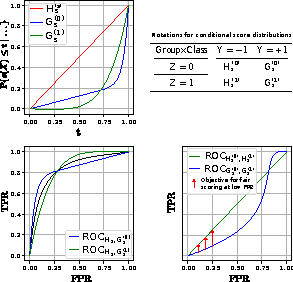
\includegraphics[width=0.6\columnwidth]{images/original_paper/example_simple_dists_explained_with_table2.pdf}
        \caption{Illustrating the limitations of $AUC$-based fairness.}
        \label{fig:example-1}
    \end{figure}
\end{frame}

\subsection{ROC based constraints}
\begin{frame}{ROC based constraints}
    
\end{frame}
